\begin{figure}[h]
    \centering
    \definecolor{clrMental}{HTML}{4E79A7}
    \definecolor{clrTemporal}{HTML}{F28E2B}
    \definecolor{clrPerformance}{HTML}{59A14F}
    \definecolor{clrEffort}{HTML}{E15759}
    \definecolor{clrFrustration}{HTML}{B07AA1}
    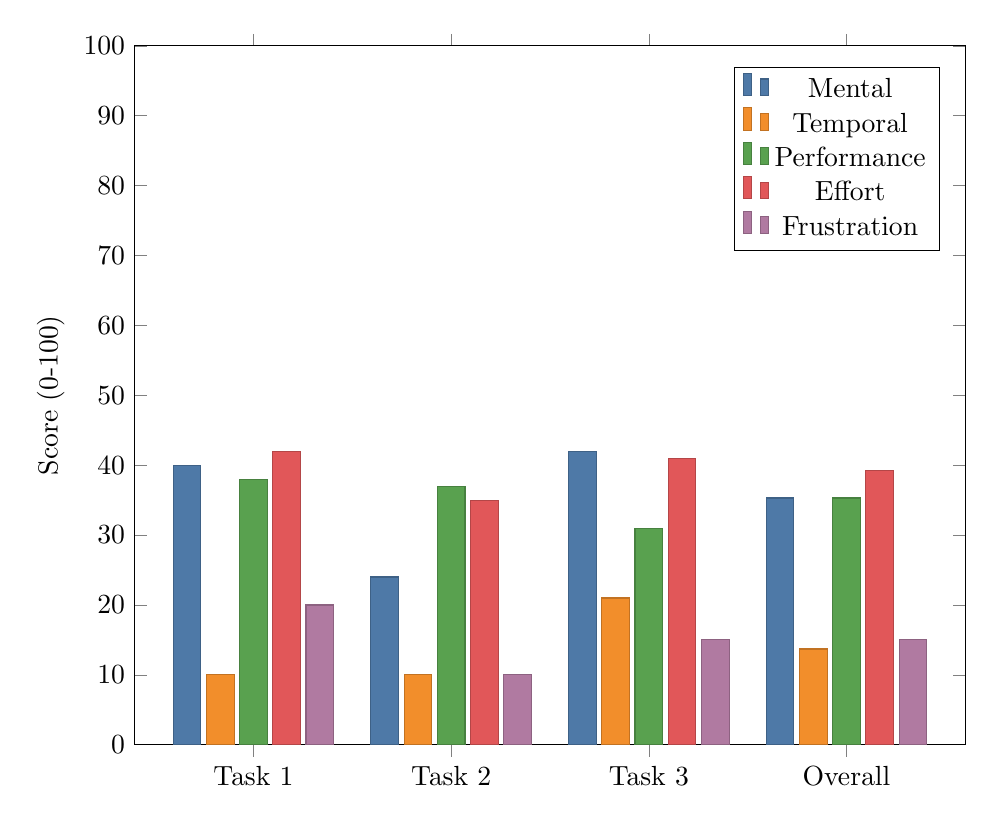
\begin{tikzpicture}
        \begin{axis}[
            ybar,
            compat=1.18,
            width=\linewidth,
            ylabel={Score (0-100)},
            ymin=0,
            ymax=100,
            symbolic x coords={Task 1, Task 2, Task 3, Overall},
            xtick=data,
            enlarge x limits=0.2,
            legend pos=north east,
        ]
        % Mental Demand
        \addplot[fill=clrMental, draw=clrMental!80!black] coordinates {(Task 1, 40.0) (Task 2, 24.0) (Task 3, 42.0) (Overall, 35.3)};
        % Temporal Demand
        \addplot[fill=clrTemporal, draw=clrTemporal!80!black] coordinates {(Task 1, 10.0) (Task 2, 10.0) (Task 3, 21.0) (Overall, 13.7)};
        % Performance
        \addplot[fill=clrPerformance, draw=clrPerformance!80!black] coordinates {(Task 1, 38.0) (Task 2, 37.0) (Task 3, 31.0) (Overall, 35.3)};
        % Effort
        \addplot[fill=clrEffort, draw=clrEffort!80!black] coordinates {(Task 1, 42.0) (Task 2, 35.0) (Task 3, 41.0) (Overall, 39.3)};
        % Frustration
        \addplot[fill=clrFrustration, draw=clrFrustration!80!black] coordinates {(Task 1, 20.0) (Task 2, 10.0) (Task 3, 15.0) (Overall, 15.0)};
        

        \legend{Mental, Temporal, Performance, Effort, Frustration}
        \end{axis}
    \end{tikzpicture}
    \caption{Subscale means for each task}
    \label{fig:tlx-task-subscales}
\end{figure}